\subsection{Obstacle width}
\label{sec:res-width}

Width (5 vs 15\,cm, chance 50\,\%) is recognised only slightly above chance with any input or model: 54--65\,\% with the Dot
summary features (Table~\ref{tab:limbs}) and at most 66\,\% with new width-specific features (Table~\ref{tab:explorewidth}).
The generic model recognises the 5\,cm obstacle in 62\,\% and the 15\,cm one in 53\,\% of crossings (Figure~\ref{fig:confusion}, right).
For all six obstacles, person scaling reaches 61\,\% (chance 17\,\%); the errors are almost all between the two widths of the
same height (Table~\ref{tab:sixconf}).

\begin{table}[htbp]
\centering
\caption{Width with new features (person scaling): clearance-shape features, step-relative ratios and their combination.}
\label{tab:explorewidth}
\begin{adjustbox}{max width=\textwidth}
{\footnotesize
\begin{tabular}{lllrrr}
\toprule
\textbf{features} & \textbf{norm} & \textbf{model} & \textbf{lead} & \textbf{trail} & \textbf{fusion} \\
\midrule
summary & self & logreg & 64.6\% (63--67; worst 60\%) & 58.5\% (53--65; worst 46\%) & 64.3\% (59--69; worst 50\%) \\
summary & self & boost & 60.9\% (56--66; worst 48\%) & 60.4\% (56--65; worst 46\%) & 61.2\% (56--67; worst 46\%) \\
shape & self & logreg & 56.8\% (51--61; worst 41\%) & 64.6\% (59--71; worst 52\%) & 64.6\% (58--71; worst 44\%) \\
ratio & self & logreg & 59.5\% (52--65; worst 37\%) & 60.2\% (55--66; worst 45\%) & 62.6\% (56--68; worst 42\%) \\
ratio + summary & self & logreg & 62.7\% (59--66; worst 54\%) & 62.7\% (57--69; worst 50\%) & 66.2\% (61--72; worst 57\%) \\
\bottomrule
\end{tabular}
}
\end{adjustbox}

\end{table}

\begin{table}[htbp]
\centering
\caption{Six-obstacle confusion matrix (person scaling, forest, soft vote; rows = true obstacle W[width]H[height]).}
\label{tab:sixconf}
\begin{adjustbox}{max width=\textwidth}
{\footnotesize
\begin{tabular}{lrrrrrr}
\toprule
\textbf{true \textbackslash{}\textbackslash{} pred} & \textbf{W1H1} & \textbf{W1H2} & \textbf{W1H3} & \textbf{W2H1} & \textbf{W2H2} & \textbf{W2H3} \\
\midrule
W1H1 & 32 & 0 & 0 & 12 & 0 & 0 \\
W1H2 & 0 & 24 & 3 & 1 & 13 & 1 \\
W1H3 & 0 & 2 & 20 & 0 & 5 & 14 \\
W2H1 & 15 & 3 & 0 & 26 & 0 & 0 \\
W2H2 & 0 & 14 & 7 & 0 & 27 & 0 \\
W2H3 & 0 & 0 & 10 & 0 & 1 & 30 \\
\bottomrule
\end{tabular}
}
\end{adjustbox}

\end{table}

\paragraph{Is the limit the sensor or the behaviour?} The camera sees where the feet are placed relative to the obstacle, which
the IMUs cannot. Even so, the 10\,cm wider obstacle changes the foot placement by only a few centimetres (crossing step
+37\,mm, Table~\ref{tab:storywidth}), and width classified from the camera foot placement reaches only 57.6\,\%. The side-to-side
(out-of-plane) motion of the thigh, shank and foot does not help either (Table~\ref{tab:lateral}, Figure~\ref{fig:lateral}).
The width limit is therefore behavioural: people cross a 5 and a 15\,cm deep obstacle in almost the same way.

\begin{table}[htbp]
\centering
\caption{Effect of width on the foot placement seen by the camera and on the Dot trajectory (W2 $-$ W1, median over participants).}
\label{tab:storywidth}
\begin{adjustbox}{max width=\textwidth}
{\footnotesize
\begin{tabular}{p{5.6cm}rrrr}
\toprule
\textbf{variable} & \textbf{W2 - W1 (median over participants)} & \textbf{range} & \textbf{participants $>$ 0} & \textbf{$\eta^2$ width} \\
\midrule
trail toe before obstacle centre (camera) & +30 mm & $-$21 to +75 & 9 / 10 & 0.05 \\
lead heel after obstacle centre (camera) & +5 mm & $-$82 to +81 & 6 / 10 & 0.00 \\
crossing step, trail toe $\rightarrow$ lead heel (camera) & +37 mm & $-$59 to +65 & 8 / 10 & 0.02 \\
lead toe before centre at its toe-off (camera) & +76 mm & $-$122 to +237 & 7 / 10 & 0.02 \\
trail heel after obstacle centre (camera) & $-$8 mm & $-$54 to +53 & 4 / 10 & 0.00 \\
lead foot apex progression (Dot) & +55 mm & $-$7 to +227 & 7 / 10 & 0.04 \\
lead landing progression (Dot) & +31 mm & $-$87 to +84 & 6 / 10 & 0.01 \\
trail landing progression (Dot) & +37 mm & $-$7 to +86 & 8 / 10 & 0.05 \\
lead $\rightarrow$ trail apex lag (Dot) & +14 ms & $-$29 to +57 & 6 / 10 & 0.01 \\
\bottomrule
\end{tabular}
}
\end{adjustbox}

\end{table}

\paragraph{Side-to-side motion.} A wider obstacle might change the frontal-plane tilt, the twist of the segments or the foot's
sideways path instead of the sagittal motion. It does not: the largest width effect on any out-of-plane feature is 6\,\% of the
within-person variance (Table~\ref{tab:lateral}), width from the out-of-plane features alone is 53--54\,\%, and adding them to the
sagittal features does not improve width or height (Table~\ref{tab:lateralclass}). Figure~\ref{fig:lateral} compares the width
effect sizes of the sagittal and out-of-plane features.

\begin{table}[htbp]
\centering
\caption{Width effect on the out-of-plane features ($\eta^2$ within participant $\times$ height), with the W2 $-$ W1 difference and
the height effect for comparison.}
\label{tab:lateral}
\begin{adjustbox}{max width=\textwidth}
{\footnotesize
\begin{tabular}{lrrrr}
\toprule
\textbf{feature} & \textbf{$\eta^2$ width} & \textbf{W2 - W1 (median)} & \textbf{participants $>$ 0} & \textbf{$\eta^2$ height (within person)} \\
\midrule
\texttt{trail\_\allowbreak{}thigh\_\allowbreak{}fr\_\allowbreak{}meandev} & 0.06 & $-$0.97 & 2 / 10 & 0.17 \\
\texttt{lead\_\allowbreak{}foot\_\allowbreak{}path\_\allowbreak{}ratio} & 0.05 & +0.01 & 8 / 10 & 0.32 \\
\texttt{trail\_\allowbreak{}shank\_\allowbreak{}fr\_\allowbreak{}maxdev} & 0.03 & +2.39 & 8 / 10 & 0.13 \\
\texttt{lead\_\allowbreak{}foot\_\allowbreak{}lat\_\allowbreak{}out} & 0.03 & +8.12 & 9 / 10 & 0.12 \\
\texttt{trail\_\allowbreak{}shank\_\allowbreak{}fr\_\allowbreak{}range} & 0.03 & +2.27 & 8 / 10 & 0.10 \\
\texttt{trail\_\allowbreak{}thigh\_\allowbreak{}fr\_\allowbreak{}range} & 0.03 & +1.54 & 8 / 10 & 0.22 \\
\texttt{lead\_\allowbreak{}foot\_\allowbreak{}fr\_\allowbreak{}maxdev} & 0.03 & +1.43 & 8 / 10 & 0.01 \\
\texttt{trail\_\allowbreak{}thigh\_\allowbreak{}fr\_\allowbreak{}maxdev} & 0.03 & +1.37 & 7 / 10 & 0.24 \\
\texttt{lead\_\allowbreak{}foot\_\allowbreak{}fr\_\allowbreak{}range} & 0.02 & +1.01 & 8 / 10 & 0.01 \\
\texttt{trail\_\allowbreak{}shank\_\allowbreak{}fr\_\allowbreak{}meandev} & 0.02 & $-$1.23 & 2 / 10 & 0.12 \\
\texttt{lead\_\allowbreak{}shank\_\allowbreak{}fr\_\allowbreak{}range} & 0.02 & +1.27 & 8 / 10 & 0.08 \\
\texttt{trail\_\allowbreak{}foot\_\allowbreak{}fr\_\allowbreak{}maxdev} & 0.02 & +1.04 & 8 / 10 & 0.19 \\
\texttt{lead\_\allowbreak{}thigh\_\allowbreak{}yaw\_\allowbreak{}meandev} & 0.02 & $-$0.20 & 5 / 10 & 0.01 \\
\texttt{trail\_\allowbreak{}foot\_\allowbreak{}fr\_\allowbreak{}range} & 0.02 & +0.98 & 8 / 10 & 0.16 \\
\texttt{lead\_\allowbreak{}shank\_\allowbreak{}yaw\_\allowbreak{}maxdev} & 0.01 & $-$1.19 & 3 / 10 & 0.01 \\
\bottomrule
\end{tabular}
}
\end{adjustbox}

\end{table}

\begin{table}[htbp]
\centering
\caption{Width and height classification with out-of-plane features, original sagittal + shape features, and both (person scaling).}
\label{tab:lateralclass}
\begin{adjustbox}{max width=\textwidth}
{\footnotesize
\begin{tabular}{lp{4.6cm}lrrr}
\toprule
\textbf{target} & \textbf{features} & \textbf{model} & \textbf{lead} & \textbf{trail} & \textbf{fusion} \\
\midrule
width & out-of-plane only & logistic & 53.0\% (45--62) & 48.0\% (39--56) & 53.4\% (48--60) \\
width & out-of-plane only & forest & 53.5\% (48--60) & 48.8\% (44--53) & 53.8\% (49--59) \\
width & original sagittal + shape & logistic & 60.8\% (57--65) & 61.9\% (57--68) & 65.8\% (62--70) \\
width & original sagittal + shape & forest & 61.5\% (57--66) & 56.5\% (52--62) & 62.3\% (58--68) \\
width & sagittal + shape + out-of-plane & logistic & 59.3\% (54--65) & 56.9\% (49--66) & 61.5\% (56--69) \\
width & sagittal + shape + out-of-plane & forest & 63.0\% (56--69) & 58.4\% (54--63) & 63.4\% (57--71) \\
height & out-of-plane only & logistic & 59.7\% (52--67) & 48.7\% (40--58) & 61.4\% (55--68) \\
height & out-of-plane only & forest & 59.3\% (49--68) & 54.5\% (45--64) & 64.0\% (57--71) \\
height & original sagittal + shape & logistic & 83.4\% (77--89) & 77.3\% (66--86) & 83.0\% (77--89) \\
height & original sagittal + shape & forest & 87.7\% (82--92) & 86.5\% (78--92) & 91.5\% (86--97) \\
height & sagittal + shape + out-of-plane & logistic & 86.9\% (83--91) & 79.1\% (74--83) & 86.8\% (82--92) \\
height & sagittal + shape + out-of-plane & forest & 87.3\% (82--92) & 87.0\% (79--93) & 91.2\% (85--96) \\
\bottomrule
\end{tabular}
}
\end{adjustbox}

\end{table}

\begin{figure}[htbp]
\centering
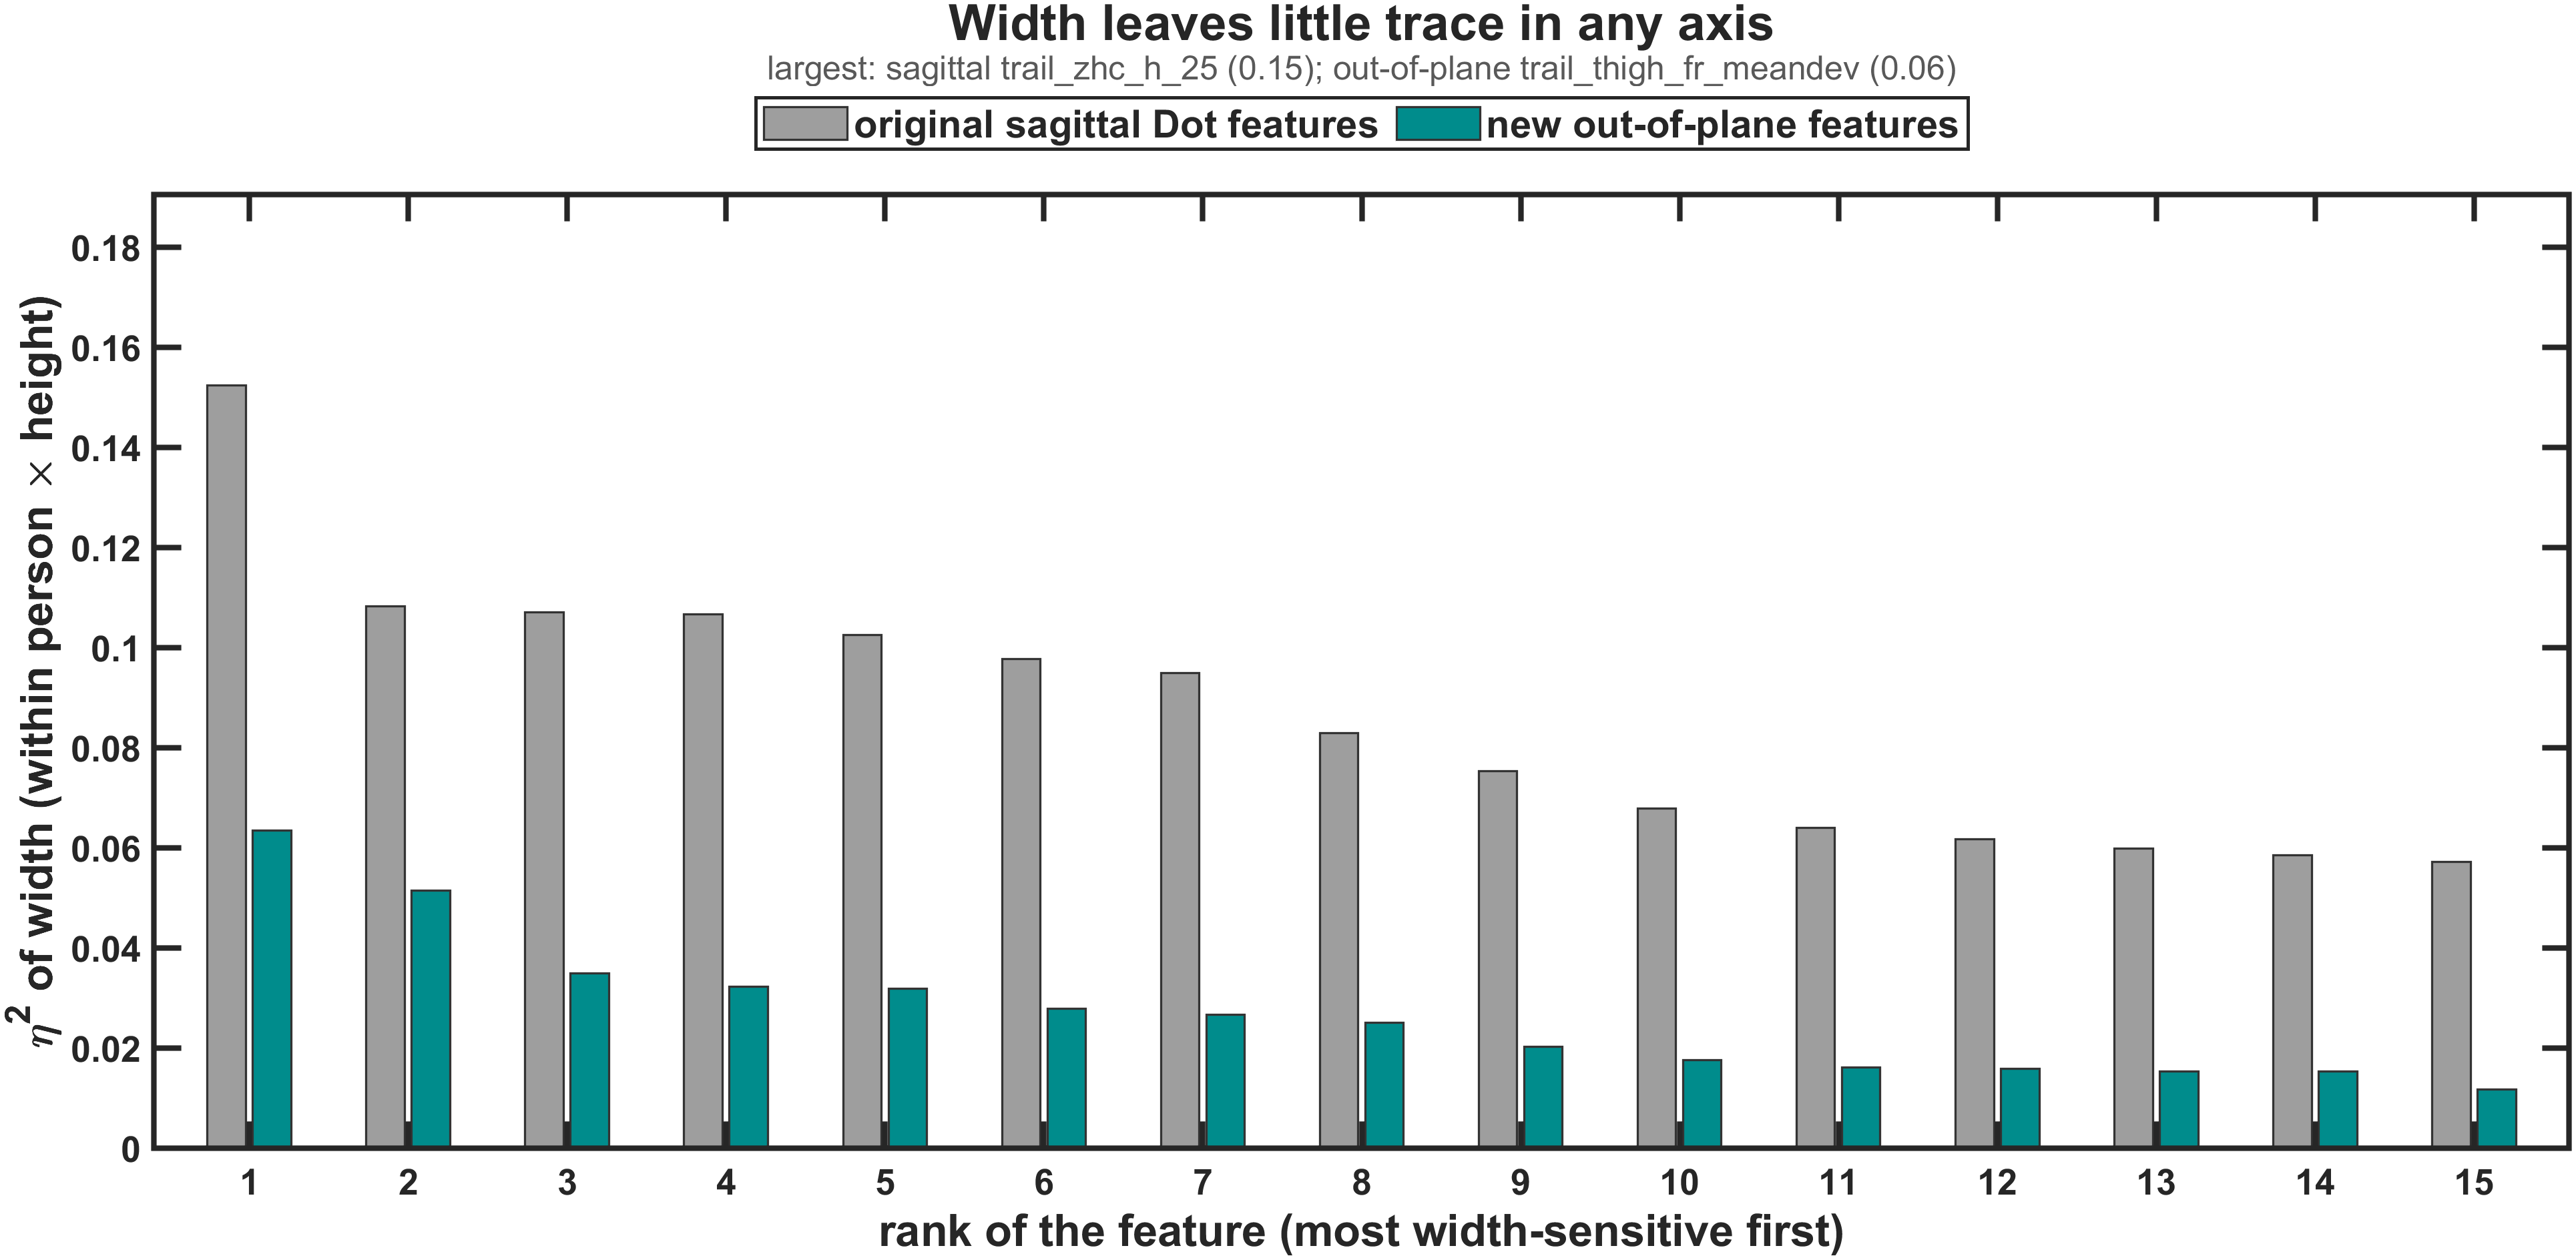
\includegraphics[width=0.9\textwidth]{fig_lateral.png}
\caption{Width effect size ($\eta^2$ within participant $\times$ height) of the 15 most width-sensitive sagittal (grey) and
out-of-plane (teal) features.}
\label{fig:lateral}
\end{figure}

